\documentclass[11pt,a4paper]{article}

\usepackage[margin=0.95in]{geometry}
\usepackage{booktabs}
\usepackage{hyperref}
\usepackage{xcolor}
\usepackage{enumitem}
\usepackage{fancyhdr}
\usepackage{graphicx}
\usepackage{tcolorbox}
\usepackage{tikz}
\usetikzlibrary{positioning,arrows.meta}
\usepackage{caption}
\usepackage{microtype}
\usepackage[T1]{fontenc}
\usepackage[utf8]{inputenc}

\hypersetup{
  colorlinks=true,
  linkcolor=blue!50!black,
  urlcolor=blue!50!black,
  pdftitle={N2S Evidence Grounding --- Simple Guide},
  pdfauthor={CXR evidence-grounding lab}
}

\definecolor{muted}{HTML}{57534E}
\definecolor{paper}{HTML}{FFFDF8}
\definecolor{teal}{HTML}{0F766E}
\definecolor{ink}{HTML}{1C1917}

\pagestyle{fancy}
\fancyhf{}
\fancyhead[L]{\small N2S lab --- simple guide}
\fancyhead[R]{\small Companion to progress notes}
\fancyfoot[C]{\thepage}
\renewcommand{\headrulewidth}{0.3pt}

\setlist[itemize]{leftmargin=1.3em,itemsep=0.2em,topsep=0.35em}
\setlist[enumerate]{leftmargin=1.3em,itemsep=0.2em,topsep=0.35em}

\begin{document}

\begin{center}
{\LARGE\bfseries How neural meets symbolic}\\[0.35em]
{\large A simple guide to this lab (and the online demo)}\\[0.7em]
{\color{muted} Short companion to the full progress notes --- for readers new to neuro-symbolic AI.}\\[0.45em]
{\small Demo: \url{https://udonsikalu.github.io/cxr-evidence-grounding-lab/}}\\[0.2em]
{\small Full record: \texttt{notes/progress-notes.pdf}}
\end{center}

\vspace{0.5em}
\begin{tcolorbox}[colback=paper,colframe=black!18,boxrule=0.4pt,arc=2pt,left=8pt,right=8pt,top=6pt,bottom=6pt]
\textbf{Read this if} you want the idea in plain language, then open the demo.\\
\textbf{Read the full notes if} you want every protocol number, held-out table, and freeze date.
\end{tcolorbox}

\section{The idea in one picture}

\begin{center}
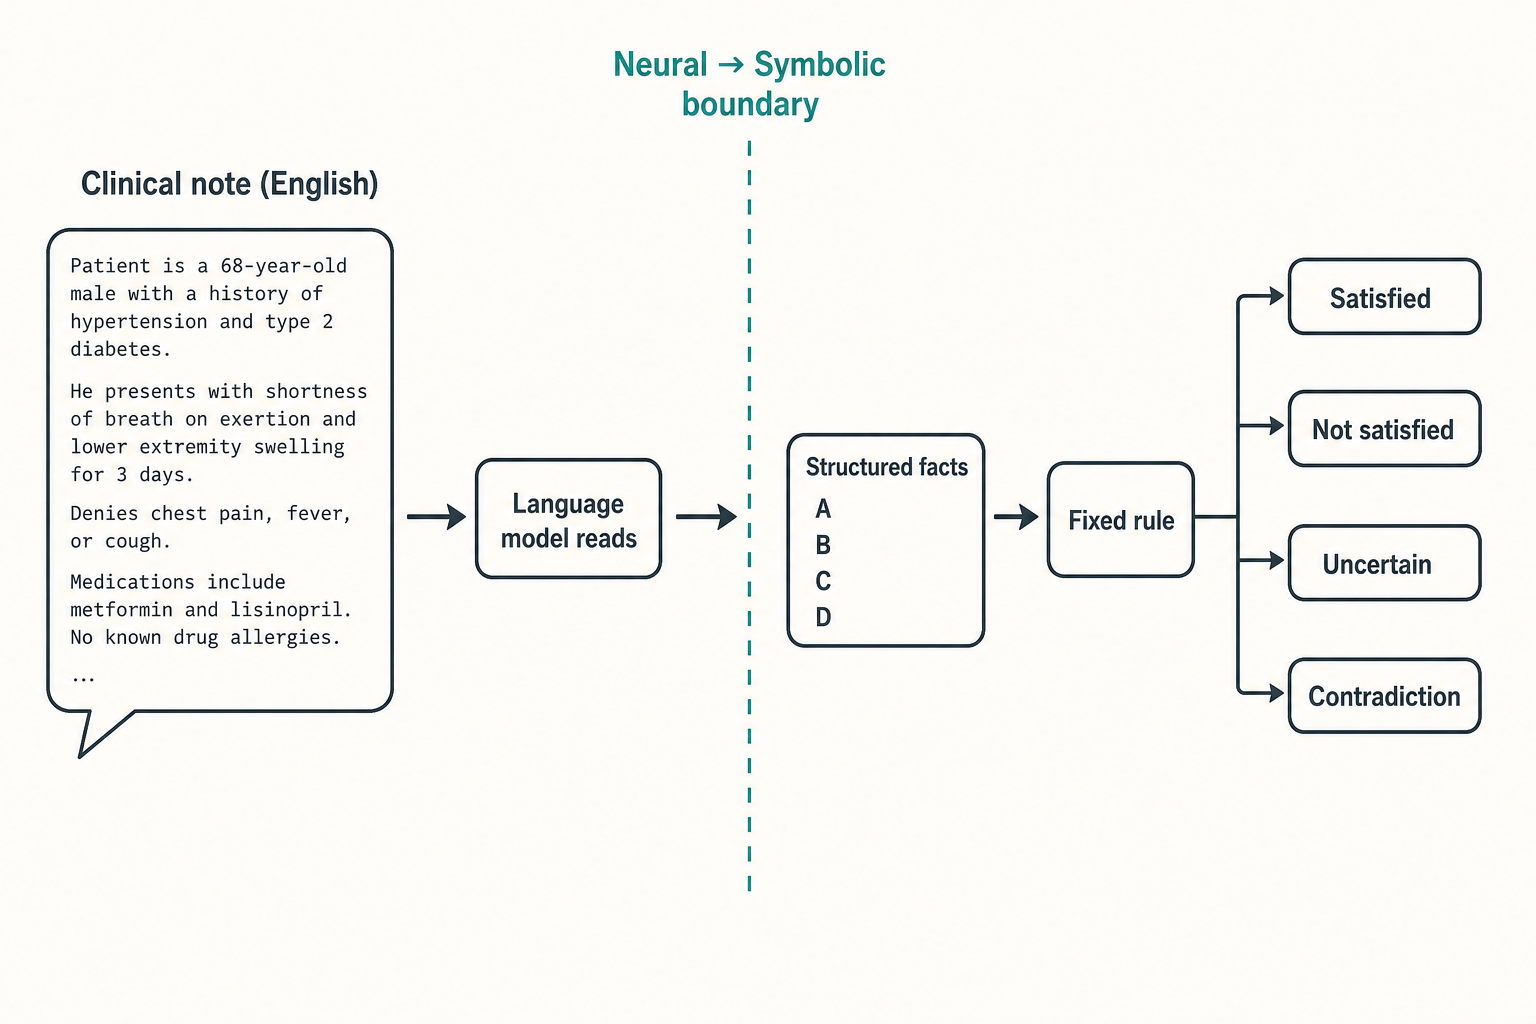
\includegraphics[width=0.92\textwidth]{figures/nesy-boundary-simple.png}
\captionof{figure}{A language model reads the note. Structured facts cross a boundary into a fixed rule. The rule --- not the model --- issues the final label.}
\end{center}

\textbf{Neuro-symbolic} means: neural (the model) + symbolic (clear rules).
The interesting failure is not ``the model is dumb.''
It is: \emph{the model seemed to understand, but the formal structure dropped the point.}

\section{Our toy question}

One made-up clinical question (synthetic notes, not real patients):

\begin{quote}
Did \textbf{first-line therapy fail}?
\end{quote}

A fixed rule needs four facts (and a contradiction flag):

\begin{center}
\begin{tabular}{@{}ll@{}}
\toprule
\textbf{Atom} & \textbf{Plain meaning} \\
\midrule
A & A first-line therapy is named \\
B & It was actually given / tried \\
C & Something counts as failure \\
D & That failure is of \emph{that} first-line regimen \\
X & The note contradicts itself about the above \\
\bottomrule
\end{tabular}
\end{center}

\vspace{0.4em}
Same atoms in $\rightarrow$ same verdict out: Satisfied, Not satisfied, Uncertain, or Contradiction.

\section{Two ways to answer the same note}

\begin{center}
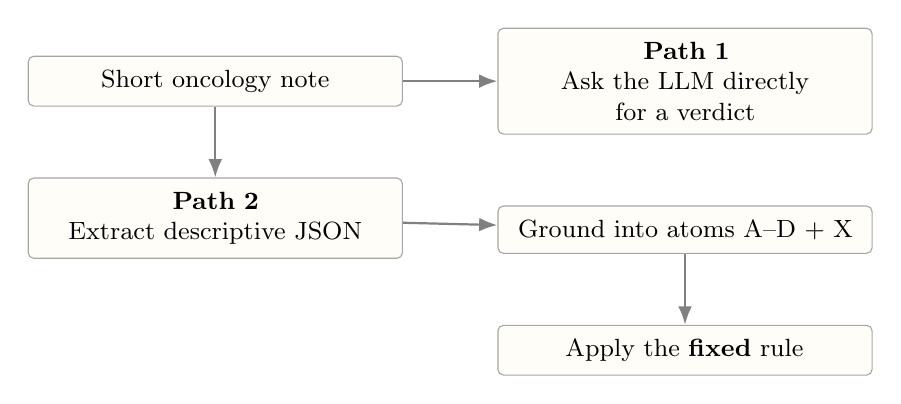
\begin{tikzpicture}[
  font=\small,
  box/.style={draw=black!35, fill=paper, align=center, inner sep=5pt, rounded corners=2pt, text width=4.4cm},
  arr/.style={-{Latex}, thick, black!50}
]
\node[box] (n) {Short oncology note};
\node[box, right=1.2cm of n] (a) {\textbf{Path 1}\\Ask the LLM directly\\for a verdict};
\node[box, below=0.9cm of n] (b1) {\textbf{Path 2}\\Extract descriptive JSON};
\node[box, below=0.9cm of a] (b2) {Ground into atoms A--D + X};
\node[box, below=0.9cm of b2] (b3) {Apply the \textbf{fixed} rule};
\draw[arr] (n) -- (a);
\draw[arr] (n) -- (b1);
\draw[arr] (b1) -- (b2);
\draw[arr] (b2) -- (b3);
\end{tikzpicture}
\captionof{figure}{We always compare both paths on the same note. Gold labels are never shown to the model.}
\end{center}

If Path~1 and Path~2 disagree, something was lost at the boundary.

\section{What the online demo shows}

The public page is \textbf{replay only}: it loads frozen experiment files.
It does \textbf{not} run a model on anyone's computer.

\begin{center}
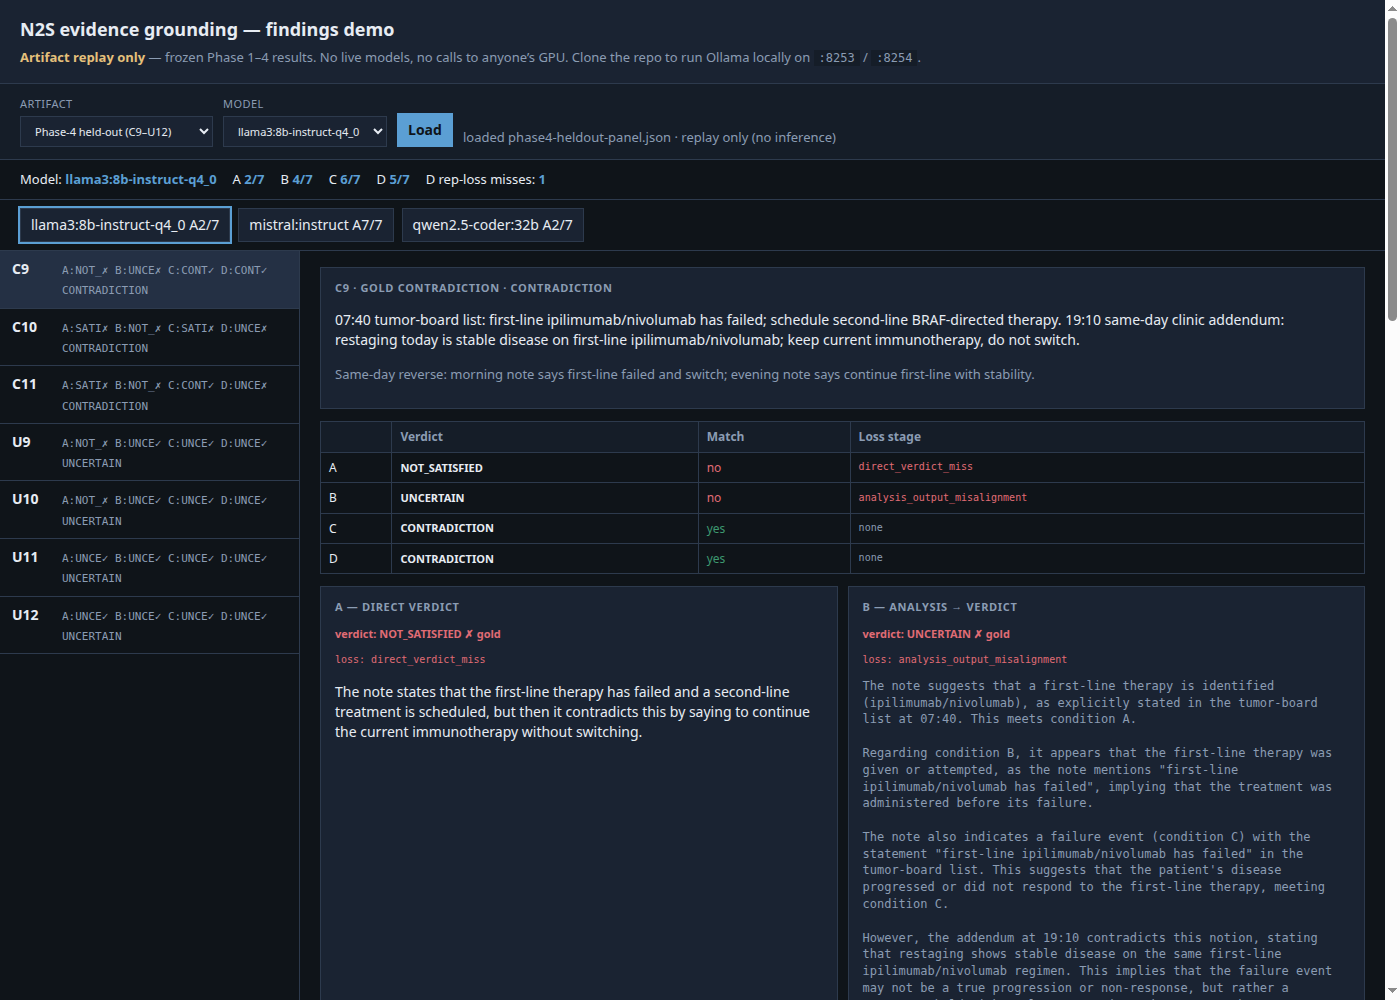
\includegraphics[width=\textwidth]{figures/demo-pages.png}
\captionof{figure}{GitHub Pages demo --- pick an artifact and a model, then click cases in the left list. Live URL: \url{https://udonsikalu.github.io/cxr-evidence-grounding-lab/}}
\end{center}

\subsection How to walk the demo (2 minutes)

\begin{enumerate}
  \item Open the link above (or open \texttt{docs/} locally).
  \item Keep the default \textbf{Phase-4} artifact, or try Phase-2 / Phase-3.
  \item Click the model buttons (Llama / Mistral / Qwen) --- same notes, different models.
  \item Click a case on the left. Read the note, then the A--D table.
\end{enumerate}

\subsection What A--D mean in the demo

These are \textbf{not} four medical rules.
They are four places meaning can disappear:

\begin{center}
\begin{tabular}{@{}p{1.2cm}p{11.2cm}@{}}
\toprule
\textbf{Col.} & \textbf{Plain meaning} \\
\midrule
\textbf{A} & Direct LLM verdict (no structure). \\
\textbf{B} & Model writes an analysis, then a final answer --- does the answer keep what the analysis said? \\
\textbf{C} & Full pipeline: extract $\rightarrow$ atoms $\rightarrow$ fixed rule. \\
\textbf{D} & Analysis had the distinction, but the \textbf{structured form} dropped it
           (``representation loss''). \\
\bottomrule
\end{tabular}
\end{center}

\vspace{0.35em}
\textbf{Loss stage} under each column tells you \emph{where} it broke, not just that it missed gold.

\begin{center}
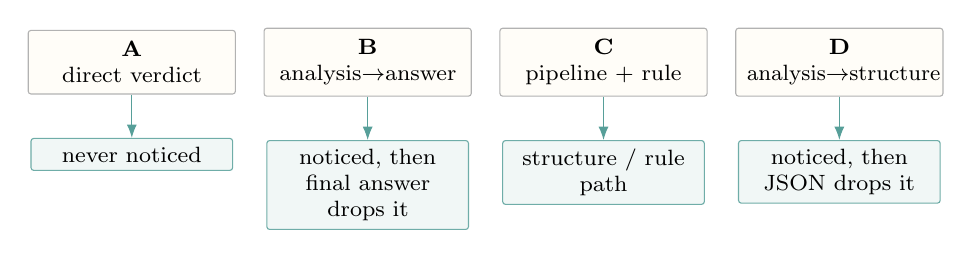
\begin{tikzpicture}[
  font=\footnotesize,
  box/.style={draw=black!30, fill=paper, align=center, inner sep=4pt, rounded corners=1pt, text width=2.35cm},
  loss/.style={draw=teal!60, fill=teal!6, align=center, inner sep=3pt, rounded corners=1pt, text width=2.35cm}
]
\node[box] (a) {\textbf{A}\\direct verdict};
\node[box, right=0.35cm of a] (b) {\textbf{B}\\analysis$\rightarrow$answer};
\node[box, right=0.35cm of b] (c) {\textbf{C}\\pipeline + rule};
\node[box, right=0.35cm of c] (d) {\textbf{D}\\analysis$\rightarrow$structure};
\node[loss, below=0.55cm of a] (la) {never noticed};
\node[loss, below=0.55cm of b] (lb) {noticed, then\\final answer drops it};
\node[loss, below=0.55cm of c] (lc) {structure / rule\\path};
\node[loss, below=0.55cm of d] (ld) {noticed, then\\JSON drops it};
\draw[-{Latex}, teal!70] (a) -- (la);
\draw[-{Latex}, teal!70] (b) -- (lb);
\draw[-{Latex}, teal!70] (c) -- (lc);
\draw[-{Latex}, teal!70] (d) -- (ld);
\end{tikzpicture}
\captionof{figure}{Conditions A--D map to different failure stories. That is why the demo shows all four.}
\end{center}

\section{The story in three beats}

\begin{enumerate}
  \item \textbf{Make the boundary visible.} Same notes, direct LLM vs structured pipeline (Milestone~1 UI on port 8253 if you run locally).
  \item \textbf{Keep hard states on purpose.} Mark contradiction and uncertainty in the structured form so the rule can fire --- states the raw LLM often narrates and then throws away.
  \item \textbf{Ask where meaning died.} Conditions A--D on discovery notes, then held-out notes, across three local models. Representation loss (D) still appeared on unseen wording.
  \item \textbf{Verify, then abstain safely (Phase~5).} If structured form may not match what the analysis said, regenerate once; if still unverifiable, emit \textbf{Review} --- not a guessed verdict, and not the same as clinical Uncertain.
  \item \textbf{Stack more checks (Phase~6--7).} Round-trip + dual-path, then an evidence span gate; try the same idea on BMT/CAR-T wording. Safer auto-labels often mean more Reviews.
  \item \textbf{Rep-eng pilot (Phase~9--10).} On one BMT false-contradiction case: localize the repair commit, then show hidden activation steering (not logit bias) can flip the model's contradiction choice while controls hold.
\end{enumerate}

That is the arc. The long PDF lists every count and protocol freeze.

\section{Phase~5 in one sentence}

When the model's JSON might have dropped what its own analysis noticed, the system checks, tries once to repair, then either applies the fixed rule or says \textbf{Review}.
On the Phase~4 held-out slice, every measured D ``representation loss'' was either fixed or sent to Review --- not left as a silent wrong label.

\section{Phase~6--7 in one sentence}

Phase~6: if two paths disagree or a paraphrase of the structure does not match the note, Review.
Phase~7: every formal claim must carry a source span; same stack on six BMT/CAR-T notes --- Llama/Mistral Dual\_full safety 1.0 (lower coverage); Qwen coder 0.75; evidence gate barely moved the needle. Soft claim only.

\section{Phase~8 in one sentence}

A mid Qwen 2.5 14B and a non-coder Qwen 2.5 32B were run on the same safety stack.
On BMT/CAR-T, non-coder 32B Dual safety reached 1.0 (vs frozen coder 0.75); 14B still missed once. Size helps some; protocol still required. Soft claim only.

\section{Phase~9 in plain language (rep-eng pilot, frozen Aug 2026)}

\textbf{Problem case BC\_E1:} a note describes response then progression (normal course). Gold = Satisfied. Some models still mark \textbf{contradiction.present = true} after repair and can AUTO-label Contradiction --- wrong.

\textbf{What we did (Observe $\rightarrow$ Localize $\rightarrow$ Intervene):}
\begin{itemize}
  \item \textbf{9A:} Same note + schema on HuggingFace Qwen 7B vs 14B. 7B repair sets X=true; 14B stays false.
  \item \textbf{9B:} At the repair step where the model writes \texttt{present: true/false}, 7B logit margin favored true (+1.6); 14B favored false ($-$4.0).
  \item \textbf{9C:} We added +4 logit bias toward \texttt{false} \emph{only at that commit}. BC\_E1 flipped to X=false and verdict Satisfied. Two control cases unchanged.
\end{itemize}

\textbf{What that proves:} the error is causally tied to the \textbf{repair boolean commit}, not immovable.

\textbf{What Phase~9 alone did \emph{not} prove:} hidden-representation steering (9C used logit bias). \textbf{Phase~10} (below) addressed that.

\section{Phase~10 (frozen Aug 2026 --- genuine pilot rep-eng)}

\textbf{Stricter question answered:} yes --- on BC\_E1, patching hidden layers at the repair commit (no logit bias) made 7B \emph{naturally} commit \texttt{false}.

\textbf{Method:} fixed direction = BC\_E2 false-commit hidden minus BC\_E1 true-commit hidden, layers 0.75 + 1.00; patch only at \texttt{contradiction.present} commit.

\textbf{Result @ $\alpha$=4:} logit margin +1.6 $\rightarrow$ $-$0.1; X true$\rightarrow$false; verdict Contradiction$\rightarrow$Satisfied. Controls BC\_C1 / BC\_E2 unchanged.

\textbf{Claim (pilot):} contrast-derived hidden patch \textbf{causally changed} classification on BC\_E1 while preserving two controls.

\textbf{Do not overclaim:} we found a \emph{steerable direction}, not ``the contradiction representation.'' One case; $\alpha$ tuned on target.

Next: Phase~11 --- does the \textbf{same frozen vector} generalize?

\section{Phase~11 (frozen Aug 2026 --- partial generalization)}

\textbf{Question:} same Ph10 vector + $\alpha$=4 on \textbf{unseen} held-out notes?

\textbf{Result:} gate \textbf{NO} but informative --- controls 3/3 held; BC11\_E2 fixed; BC11\_E3 still wrong (margin dropped only).

\textbf{Reading:} direction generalizes to at least one unseen course case; not universal. Freeze as soft partial result.

Artifact: \texttt{artifacts/phase11-generalization-panel.json}. Explorer: \url{http://127.0.0.1:8256/} (\texttt{cxr-evidence-grounding-lab-repeng/}).

\section{Phase~12A (frozen Aug 2026 --- margin / strength regime)}

\textbf{Question:} Ph11's miss on E3 --- wrong direction, or same direction but not strong enough?

\textbf{Method:} same frozen Ph10 vector; $\alpha\in\{2,4,6,8\}$ on BC11\_E2 and BC11\_E3; controls stay at $\alpha$=4.

\textbf{Result:} mechanism gate \textbf{YES}. Margins move monotonically toward \texttt{false}. E2 flips at $\alpha$=4 (baseline margin $+1.13$). E3 flips at $\alpha$=8 (baseline $+2.38$).

\textbf{Reading:} Ph11 and Ph12 are complementary. Fixed $\alpha$=4 was too weak for E3; the direction still works. Soft claim on these two cases only --- not ``all failures are margin-regime.'' Freeze before adaptive-$\alpha$ experiments.

Artifact: \texttt{artifacts/phase12-margin-regime-panel.json}. Protocol: \texttt{docs/PHASE12-PROTOCOL.md}.

\section{Phase~12B (frozen Aug 2026 --- second held-out; gate NO)}

\textbf{Question:} does Ph12A's LOW/HIGH $\alpha$ rule transfer to \textbf{new} notes?

\textbf{Result:} gate \textbf{NO}. All three targets HIGH; margins moved toward false but none flipped by $\alpha$=8. Contradiction control BC12\_C1 broken at $\alpha$=4 (true$\rightarrow$false). N1 held.

\textbf{Reading:} direction still has leverage; ``HIGH $\Rightarrow$ flip @8'' did not transfer; more strength is not free. Soft negative --- freeze before adaptive-$\alpha$.

Artifact: \texttt{artifacts/phase12b-heldout-panel.json}. Protocol: \texttt{docs/PHASE12B-PROTOCOL.md}.

\section{Phase~13 (frozen Aug 2026 --- representation geometry; gate YES)}

\textbf{Question:} at the repair commit (no steer), do course false-X notes and true-contradiction notes sit in separable regions along the Ph10 direction?

\textbf{Result:} gate \textbf{YES} (soft). 5/5 course + 4/4 contradiction usable. cos@1.00 ranges do not overlap (gap $\approx 0.021$). Leave-one-out probe accuracy $0.889$.

\textbf{Reading:} classes look softly separable --- useful for designing safer conditional interventions later. Does \textbf{not} by itself authorize adaptive-$\alpha$. Soft pilot only.

Artifact: \texttt{artifacts/phase13-geometry-panel.json}. Protocol: \texttt{docs/PHASE13-PROTOCOL.md}.

\section{Phase~14 (frozen Aug 2026 --- gated steer; gate NO)}

\textbf{Question:} can a frozen cosine gate ($\tau{=}{-}0.690$ from Ph13) decide when to apply Ph10 steer at $\alpha$=4 on \textbf{new} notes?

\textbf{Result:} gate \textbf{NO}. Contradiction controls and N1 stayed STEER OFF. Only 1/3 course crossed $\tau$; that case moved margin but did not flip X. Utility flips = 0.

\textbf{Reading:} soft negative --- this $\tau{+}\alpha$=4 recipe is not a sufficient conclusion of the Ph9--13 arc. Freeze; do not retune on this held-out or jump to adaptive-$\alpha$.

Artifact: \texttt{artifacts/phase14-gated-panel.json}. Protocol: \texttt{docs/PHASE14-PROTOCOL.md}.

\section{What we are (and are not) claiming}

\begin{itemize}
  \item \textbf{Are:} a small synthetic lab that makes the neural$\rightarrow$symbolic handoff \emph{inspectable}.
  \item \textbf{Are not:} a clinical product, a medical device, or the full CXR stack (no Qdrant / Archetypes here).
  \item \textbf{Public demo:} frozen files only --- safe to share; no inference on the author's servers.
\end{itemize}

\section{Where to go next}

\begin{center}
\begin{tabular}{@{}ll@{}}
\toprule
\textbf{Want\ldots} & \textbf{Open\ldots} \\
\midrule
Click around & \url{https://udonsikalu.github.io/cxr-evidence-grounding-lab/} \\
Every number \& freeze & \texttt{notes/progress-notes.pdf} \\
Phase~9 simple notes & \texttt{docs/PHASE9-NOTES-SIMPLE.md} \\
Phase~10 (activation steer) & \texttt{docs/PHASE10-PROTOCOL.md} \\
Rep-eng explorer & \url{http://127.0.0.1:8256/} (\texttt{cxr-evidence-grounding-lab-repeng/}) \\
Phase~11 generalization & \texttt{docs/PHASE11-PROTOCOL.md} \\
Phase~12A margin / $\alpha$ panel & \texttt{docs/PHASE12-PROTOCOL.md} \\
Phase~12B second held-out & \texttt{docs/PHASE12B-PROTOCOL.md} \\
Phase~13 geometry & \texttt{docs/PHASE13-PROTOCOL.md} \\
Phase~14 gated steer & \texttt{docs/PHASE14-PROTOCOL.md} \\
Architecture direction & \texttt{docs/ARCHITECTURE-DIRECTION.md} \\
Written journey & \texttt{EVALUATION-JOURNEY.md} \\
Run the local UI & \texttt{python3 server.py} $\rightarrow$ \texttt{http://127.0.0.1:8253/} \\
Repo README (NeSy intro) & GitHub project homepage \\
\bottomrule
\end{tabular}
\end{center}

\vspace{1em}
\begin{center}
\color{muted}\small
Rebuild: \texttt{pdflatex progress-notes-simple.tex} from the \texttt{notes/} directory.
\end{center}

\end{document}
